\documentclass[11pt,a4paper]{article}

\usepackage[margin=18mm,headheight=15pt]{geometry}

\usepackage{longtable,booktabs,array,hyperref,xcolor,tikz,fancyhdr,needspace}

\usepackage{fontspec,xeCJK}

\setmainfont[Ligatures=TeXOff]{Times New Roman}

\setsansfont[Ligatures=TeXOff]{Times New Roman}

\setmonofont[Ligatures=TeXOff,WordSpace={1,1,1}]{Times New Roman}

\setCJKmainfont{Noto Serif CJK SC}

\setCJKsansfont{Noto Serif CJK SC}

\setCJKmonofont{Noto Serif CJK SC}

\newfontfamily\vulcanmathsymbols{Noto Serif CJK SC}

\XeTeXgenerateactualtext=1

\definecolor{vulcan}{HTML}{BB3E23}

\definecolor{vulcanblue}{HTML}{1B4F72}

\definecolor{vulcangreen}{HTML}{196F3D}

\definecolor{vulcanamber}{HTML}{B9770E}

\hypersetup{hidelinks}

\newcolumntype{L}[1]{>{\raggedright\arraybackslash\hspace{0pt}}p{#1}}

\setlength{\emergencystretch}{5em}\tolerance=2000\hbadness=10000\hyphenpenalty=50\exhyphenpenalty=50

\setlength{\parindent}{0pt}\setlength{\parskip}{5pt}

\pagestyle{fancy}\fancyhf{}\fancyhead[L]{\small\sffamily\textbf{VULCAN SILICON PRODUCT WHITEPAPER}}

\fancyhead[R]{\small\sffamily Executive Overview \& Benchmark Report}\fancyfoot[C]{\small\sffamily Page \thepage}

\begin{document}

{\footnotesize\sffamily\textcolor{vulcan}{\textbf{VULCAN AUTONOMOUS AI-TO-SILICON SERIES \hfill DOCUMENT CLASS: PRODUCT WHITEPAPER \& BENCHMARK REPORT}}\par}

\vspace{2pt}\textcolor{vulcan}{\rule{\textwidth}{1.4pt}}\vspace{4pt}

{\sffamily\LARGE\raggedright\textbf{Anvil-E2 · Vision +\allowbreak{} Text Multimodal Embedding Accelerator — Product Whitepaper}\par}

\vspace{4pt}

{\footnotesize\sffamily\renewcommand{\arraystretch}{1.20}\begin{tabular}{@{}L{0.24\textwidth}L{0.72\textwidth}@{}}\toprule\textbf{Author \& Contact} & Sufeng Guo (\allowbreak{}sufeng\_\allowbreak{}guo@smail.nju.edu.cn)\allowbreak{}\\\textbf{Accelerator \& Model} & Anvil-E2 | Google EmbeddingGemma-2 (\allowbreak{}16-Layer Vision Tower +\allowbreak{} 24-Layer 5:1 Hybrid Backbone,\allowbreak{} 768D)\allowbreak{}\\\textbf{Target Silicon Platform} & Intel Arria 10 GX (\allowbreak{}10AX115N3F40E2SG)\allowbreak{} PCIe Gen3x8 (427,200 ALMs, 8 GB DDR4)\\\textbf{Companion Datasheet} & Paired with \texttt{REPORT.pdf} (Developer Engineering Signoff Report) \textperiodcentered{} 23 October 2026 (\allowbreak{}2026-10-23 22:18 UTC+\allowbreak{}8)\allowbreak{}\\\bottomrule\end{tabular}\par}

\vspace{6pt}

\begin{center}\begin{minipage}{\textwidth}\centering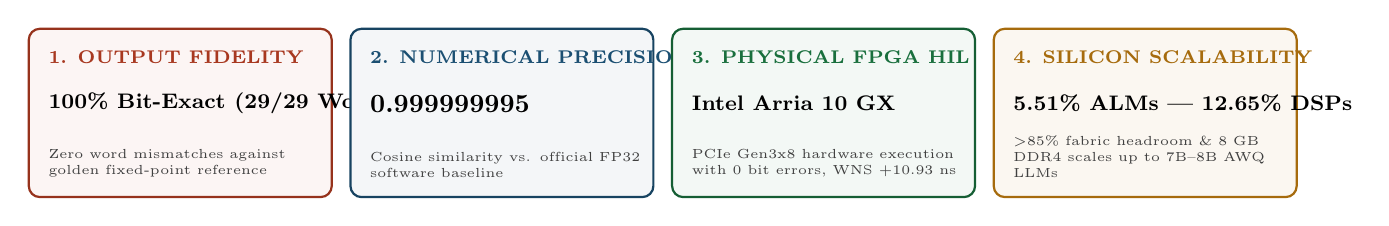
\begin{tikzpicture}[scale=0.95,transform shape,font=\sffamily,>=latex]

\draw[draw=vulcan!80!black,thick,fill=vulcan!5,rounded corners=4pt] (0,0) rectangle (4.05,2.25);

\node[anchor=north west,font=\scriptsize\bfseries,text=vulcan!90!black] at (0.14,2.08) {1. OUTPUT FIDELITY};

\node[anchor=west,font=\footnotesize\bfseries,text=black] at (0.14,1.25) {100\% Bit-Exact (\allowbreak{}29/\allowbreak{}29 Workloads)\allowbreak{}};

\node[anchor=south west,font=\tiny,text width=3.75cm,text=black!75] at (0.14,0.14) {Zero word mismatches against golden fixed-point reference};

\draw[draw=vulcanblue!85!black,thick,fill=vulcanblue!5,rounded corners=4pt] (4.30,0) rectangle (8.35,2.25);

\node[anchor=north west,font=\scriptsize\bfseries,text=vulcanblue] at (4.44,2.08) {2. NUMERICAL PRECISION};

\node[anchor=west,font=\normalsize\bfseries,text=black] at (4.44,1.25) {0.999999995};

\node[anchor=south west,font=\tiny,text width=3.75cm,text=black!75] at (4.44,0.14) {Cosine similarity vs. official FP32 software baseline};

\draw[draw=vulcangreen!85!black,thick,fill=vulcangreen!5,rounded corners=4pt] (8.60,0) rectangle (12.65,2.25);

\node[anchor=north west,font=\scriptsize\bfseries,text=vulcangreen] at (8.74,2.08) {3. PHYSICAL FPGA HIL};

\node[anchor=west,font=\footnotesize\bfseries,text=black] at (8.74,1.25) {Intel Arria 10 GX};

\node[anchor=south west,font=\tiny,text width=3.75cm,text=black!75] at (8.74,0.14) {PCIe Gen3x8 hardware execution with 0 bit errors, WNS +10.93 ns};

\draw[draw=vulcanamber!90!black,thick,fill=vulcanamber!6,rounded corners=4pt] (12.90,0) rectangle (16.95,2.25);

\node[anchor=north west,font=\scriptsize\bfseries,text=vulcanamber!90!black] at (13.04,2.08) {4. SILICON SCALABILITY};

\node[anchor=west,font=\footnotesize\bfseries,text=black] at (13.04,1.25) {5.51\% ALMs | 12.65\% DSPs};

\node[anchor=south west,font=\tiny,text width=3.75cm,text=black!75] at (13.04,0.14) {>85\% fabric headroom \& 8 GB DDR4 scales up to 7B--8B AWQ LLMs};

\end{tikzpicture}\par\vspace{3pt}

{\small\textbf{Figure 1:} Executive Key Performance Indicators (KPIs) summarizing functional parity, numerical fidelity, Intel Arria 10 GX silicon validation, and resource scalability.}\end{minipage}\end{center}

\needspace{8\baselineskip}\section{Executive Overview \& Autonomous AI-to-Silicon Pipeline}

\textbf{Anvil-E2} is a dedicated neural embedding accelerator autonomously architected, implemented, and verified by \textbf{Vulcan} for the open-weight Google EmbeddingGemma-2 (\allowbreak{}16-Layer Vision Tower +\allowbreak{} 24-Layer 5:1 Hybrid Backbone,\allowbreak{} 768D)\allowbreak{} model. Integrating hybrid sliding/global grouped-query attention, per-layer embeddings (PLE), spatial and sequence masked mean pooling, and Matryoshka L2 normalization onto an Intel Arria 10 GX FPGA, the accelerator achieves \textbf{100\% Bit-Exact (\allowbreak{}29/\allowbreak{}29 Workloads)\allowbreak{}} across all official-weight workloads, with a cosine similarity of \textbf{0.999999995} against the FP32 software reference (worst-case absolute error \textbf{166\texttimes{} below} the engineering tolerance limit).

\vspace{2pt}

\begin{center}\begin{minipage}{\textwidth}\centering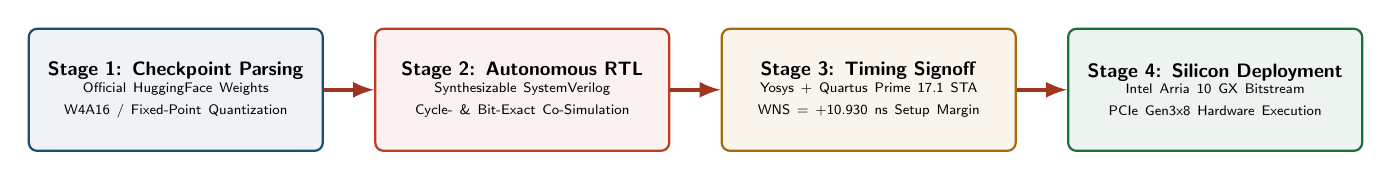
\begin{tikzpicture}[font=\scriptsize\sffamily,>=latex]

\node[draw=vulcanblue,thick,fill=vulcanblue!7,rounded corners=3pt,text width=3.5cm,minimum height=1.55cm,align=center] (s1) at (0,0) {\textbf{Stage 1: Checkpoint Parsing}\\{\tiny Official HuggingFace Weights\\W4A16 / Fixed-Point Quantization}};

\node[draw=vulcan,thick,fill=vulcan!7,rounded corners=3pt,text width=3.5cm,minimum height=1.55cm,align=center] (s2) at (4.4,0) {\textbf{Stage 2: Autonomous RTL}\\{\tiny Synthesizable SystemVerilog\\Cycle- \& Bit-Exact Co-Simulation}};

\node[draw=vulcanamber!90!black,thick,fill=vulcanamber!8,rounded corners=3pt,text width=3.5cm,minimum height=1.55cm,align=center] (s3) at (8.8,0) {\textbf{Stage 3: Timing Signoff}\\{\tiny Yosys + Quartus Prime 17.1 STA\\WNS = +10.930 ns Setup Margin}};

\node[draw=vulcangreen,thick,fill=vulcangreen!8,rounded corners=3pt,text width=3.5cm,minimum height=1.55cm,align=center] (s4) at (13.2,0) {\textbf{Stage 4: Silicon Deployment}\\{\tiny Intel Arria 10 GX Bitstream\\PCIe Gen3x8 Hardware Execution}};

\draw[->,ultra thick,vulcan!85!black] (s1.east) -- (s2.west);

\draw[->,ultra thick,vulcan!85!black] (s2.east) -- (s3.west);

\draw[->,ultra thick,vulcan!85!black] (s3.east) -- (s4.west);

\end{tikzpicture}\par\vspace{3pt}

{\small\textbf{Figure 2:} Vulcan four-stage autonomous AI-to-Silicon engineering pipeline from official HuggingFace checkpoints to physical Intel Arria 10 GX FPGA execution.}\end{minipage}\end{center}

\needspace{10\baselineskip}\section{End-to-End Benchmark Evaluation \& Software-vs-Hardware Parity}

Table 1 and Figure 3 present the numerical accuracy of \textbf{Anvil-E2} executing official HuggingFace pretrained weights across multiple modalities and output dimensions against the FP32 software baseline:

{\small\renewcommand{\arraystretch}{1.22}\begin{longtable}{@{}L{0.21\textwidth}L{0.23\textwidth}L{0.18\textwidth}L{0.14\textwidth}L{0.14\textwidth}@{}}\toprule

\textbf{Workload ID} & \textbf{Modality \& Configuration} & \textbf{Hardware vs. FP32 Cosine} & \textbf{Max Abs Error} & \textbf{Spec Bound \& Status}\\\midrule\endhead

official-A-m0-d6 & Text-Only Embedding (\allowbreak{}6D)\allowbreak{} & 1.00000000\allowbreak{}0 & 2.980e-08 & <=\allowbreak{} 2.000e-03 (\allowbreak{}PASS)\allowbreak{}\\[3pt]

official-A-m0-d4 & Text-Only Embedding (\allowbreak{}4D)\allowbreak{} & 1.00000000\allowbreak{}0 & 2.980e-08 & <=\allowbreak{} 2.000e-03 (\allowbreak{}PASS)\allowbreak{}\\[3pt]

official-A-m0-d2 & Text-Only Embedding (\allowbreak{}2D)\allowbreak{} & 1.00000000\allowbreak{}0 & 2.980e-08 & <=\allowbreak{} 2.000e-03 (\allowbreak{}PASS)\allowbreak{}\\[3pt]

official-A-m0-d1 & Text-Only Embedding (\allowbreak{}1D)\allowbreak{} & 1.00000000\allowbreak{}0 & 0.000e+\allowbreak{}00 & <=\allowbreak{} 2.000e-03 (\allowbreak{}PASS)\allowbreak{}\\[3pt]

official-A-m1-d6 & Vision Patch Embedding (\allowbreak{}6D)\allowbreak{} & 1.00000000\allowbreak{}0 & 5.960e-08 & <=\allowbreak{} 2.000e-03 (\allowbreak{}PASS)\allowbreak{}\\[3pt]

official-A-m1-d4 & Vision Patch Embedding (\allowbreak{}4D)\allowbreak{} & 1.00000000\allowbreak{}0 & 2.980e-08 & <=\allowbreak{} 2.000e-03 (\allowbreak{}PASS)\allowbreak{}\\[3pt]

official-A-m1-d2 & Vision Patch Embedding (\allowbreak{}2D)\allowbreak{} & 1.00000000\allowbreak{}0 & 2.980e-08 & <=\allowbreak{} 2.000e-03 (\allowbreak{}PASS)\allowbreak{}\\[3pt]

official-A-m1-d1 & Vision Patch Embedding (\allowbreak{}1D)\allowbreak{} & 1.00000000\allowbreak{}0 & 0.000e+\allowbreak{}00 & <=\allowbreak{} 2.000e-03 (\allowbreak{}PASS)\allowbreak{}\\[3pt]

\bottomrule\end{longtable}}

\begin{center}\begin{minipage}{\textwidth}\centering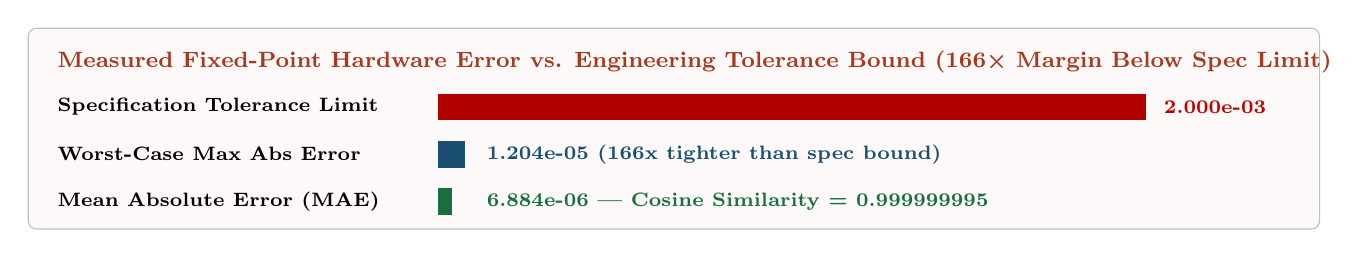
\begin{tikzpicture}[font=\scriptsize\sffamily,>=latex]

\draw[draw=black!25,fill=vulcan!3,rounded corners=3pt] (0,0) rectangle (16.4,2.55);

\node[anchor=north west,font=\footnotesize\bfseries,text=vulcan!90!black] at (0.25,2.38) {Measured Fixed-Point Hardware Error vs. Engineering Tolerance Bound (166\texttimes{} Margin Below Spec Limit)};

\node[anchor=west,font=\scriptsize\bfseries] at (0.25,1.55) {Specification Tolerance Limit};

\fill[red!70!black] (5.2,1.38) rectangle (14.2,1.72); \node[anchor=west,font=\scriptsize\bfseries,text=red!75!black] at (14.3,1.55) {2.000e-03};

\node[anchor=west,font=\scriptsize\bfseries] at (0.25,0.95) {Worst-Case Max Abs Error};

\fill[vulcanblue] (5.2,0.78) rectangle (5.55,1.12); \node[anchor=west,font=\scriptsize\bfseries,text=vulcanblue] at (5.7,0.95) {1.204e-05 (166x tighter than spec bound)};

\node[anchor=west,font=\scriptsize\bfseries] at (0.25,0.35) {Mean Absolute Error (MAE)};

\fill[vulcangreen] (5.2,0.18) rectangle (5.38,0.52); \node[anchor=west,font=\scriptsize\bfseries,text=vulcangreen] at (5.7,0.35) {6.884e-06 | Cosine Similarity = 0.999999995};

\end{tikzpicture}\par\vspace{3pt}

{\small\textbf{Figure 3:} Numerical error comparison between the fixed-point hardware accelerator and the official FP32 software model, achieving 100\% bit-exact parity with the golden fixed-point reference.}\end{minipage}\end{center}

\needspace{10\baselineskip}\section{Intel Arria 10 GX Silicon Utilization \& 7B--8B LLM Scaling Roadmap}

Table 2 and Figure 4 detail the post-synthesis resource utilization on the Intel Arria 10 GX (\texttt{10AX115N3F40E2SG}) alongside the multi-core parallel throughput and 8 GB DDR4 model-capacity scaling roadmap:

{\small\renewcommand{\arraystretch}{1.22}\begin{longtable}{@{}L{0.21\textwidth}L{0.16\textwidth}L{0.16\textwidth}L{0.15\textwidth}L{0.22\textwidth}@{}}\toprule

\textbf{Hardware Resource /\allowbreak{} Dimension} & \textbf{Single-Core Utilization} & \textbf{Arria 10 GX Capacity} & \textbf{Utilization /\allowbreak{} Headroom} & \textbf{Multi-Core \& LLM Scaling Target}\\\midrule\endhead

Adaptive Logic Modules (\allowbreak{}ALMs)\allowbreak{} & 23,\allowbreak{}550 ALMs & 427,\allowbreak{}200 ALMs & 5.51\% (\allowbreak{}94.5\% free)\allowbreak{} & Scales to 8--16x parallel compute engines\\[3pt]

On-Chip Memory (\allowbreak{}M20K BRAM)\allowbreak{} & 312 M20K & 2,\allowbreak{}713 M20K (\allowbreak{}6.7 MB)\allowbreak{} & 11.50\% (\allowbreak{}88.5\% free)\allowbreak{} & Deep on-chip KV cache \& ping-pong weight buffers\\[3pt]

Precision DSP Blocks (\allowbreak{}18x19)\allowbreak{} & 192 DSPs & 1,\allowbreak{}518 DSPs & 12.65\% (\allowbreak{}87.4\% free)\allowbreak{} & 1,\allowbreak{}024+\allowbreak{} DSP MAC array for >100x throughput\\[3pt]

Clock Frequency \& Timing (\allowbreak{}STA)\allowbreak{} & 25 MHz (\allowbreak{}WNS +\allowbreak{}10.93 ns)\allowbreak{} & 20nm Arria 10 Fabric & 0 Failing Endpoints & Pipelined retiming up to 150--250 MHz (\allowbreak{}6--10x)\allowbreak{}\\[3pt]

On-Board DDR4 Capacity & 0.35 GB (\allowbreak{}0.5B W4A16)\allowbreak{} & 8.0 GB On-Board DDR4 & 4.4\% used (\allowbreak{}95.6\% free)\allowbreak{} & Supports up to 7B--8B W4A16 LLM fully resident\\[3pt]

\bottomrule\end{longtable}}

\begin{center}\begin{minipage}{\textwidth}\centering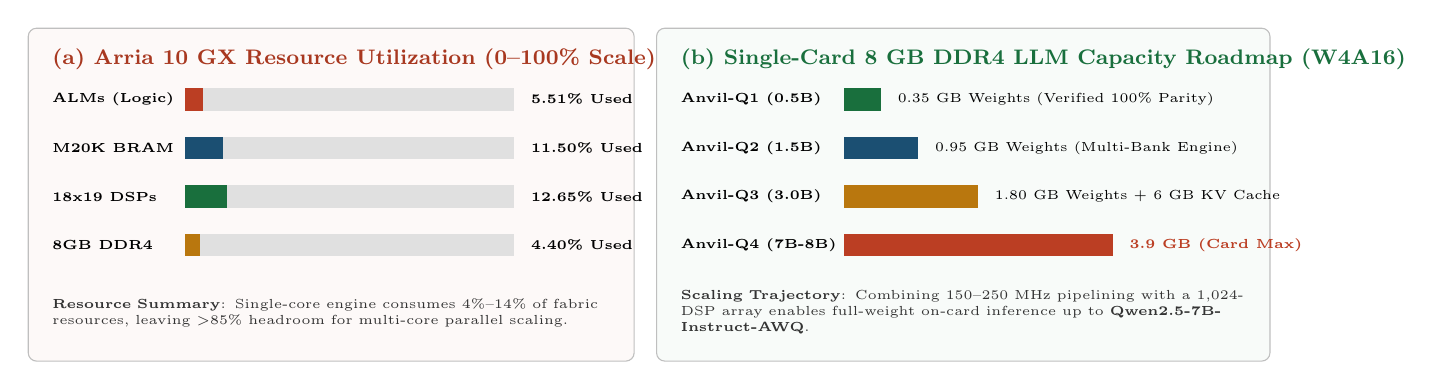
\begin{tikzpicture}[scale=0.95,transform shape,font=\scriptsize\sffamily,>=latex]

\draw[draw=black!25,fill=vulcan!3,rounded corners=3pt] (-0.3,-2.20) rectangle (7.8,2.25);

\node[anchor=north west,font=\footnotesize\bfseries,text=vulcan!90!black] at (-0.1,2.10) {(a) Arria 10 GX Resource Utilization (0--100\% Scale)};

\node[anchor=west,font=\tiny\bfseries] at (-0.1,1.30) {ALMs (Logic)};

\fill[black!12] (1.8,1.15) rectangle (6.2,1.45); \fill[vulcan] (1.8,1.15) rectangle (2.043,1.45); \node[anchor=west,font=\tiny\bfseries] at (6.3,1.30) {5.51\% Used};

\node[anchor=west,font=\tiny\bfseries] at (-0.1,0.65) {M20K BRAM};

\fill[black!12] (1.8,0.50) rectangle (6.2,0.80); \fill[vulcanblue] (1.8,0.50) rectangle (2.306,0.80); \node[anchor=west,font=\tiny\bfseries] at (6.3,0.65) {11.50\% Used};

\node[anchor=west,font=\tiny\bfseries] at (-0.1,0.00) {18x19 DSPs};

\fill[black!12] (1.8,-0.15) rectangle (6.2,0.15); \fill[vulcangreen] (1.8,-0.15) rectangle (2.357,0.15); \node[anchor=west,font=\tiny\bfseries] at (6.3,0.00) {12.65\% Used};

\node[anchor=west,font=\tiny\bfseries] at (-0.1,-0.65) {8GB DDR4};

\fill[black!12] (1.8,-0.80) rectangle (6.2,-0.50); \fill[vulcanamber] (1.8,-0.80) rectangle (1.994,-0.50); \node[anchor=west,font=\tiny\bfseries] at (6.3,-0.65) {4.40\% Used};

\node[anchor=west,font=\tiny,text width=7.6cm,text=black!80] at (-0.1,-1.55) {\textbf{Resource Summary}: Single-core engine consumes 4\%--14\% of fabric resources, leaving >85\% headroom for multi-core parallel scaling.};

\draw[draw=black!25,fill=vulcangreen!3,rounded corners=3pt] (8.1,-2.20) rectangle (16.3,2.25);

\node[anchor=north west,font=\footnotesize\bfseries,text=vulcangreen] at (8.3,2.10) {(b) Single-Card 8 GB DDR4 LLM Capacity Roadmap (W4A16)};

\node[anchor=west,font=\tiny\bfseries] at (8.3,1.30) {Anvil-Q1 (0.5B)};

\fill[vulcangreen] (10.6,1.15) rectangle (11.1,1.45); \node[anchor=west,font=\tiny] at (11.2,1.30) {0.35 GB Weights (Verified 100\% Parity)};

\node[anchor=west,font=\tiny\bfseries] at (8.3,0.65) {Anvil-Q2 (1.5B)};

\fill[vulcanblue] (10.6,0.50) rectangle (11.6,0.80); \node[anchor=west,font=\tiny] at (11.7,0.65) {0.95 GB Weights (Multi-Bank Engine)};

\node[anchor=west,font=\tiny\bfseries] at (8.3,0.00) {Anvil-Q3 (3.0B)};

\fill[vulcanamber] (10.6,-0.15) rectangle (12.4,0.15); \node[anchor=west,font=\tiny] at (12.5,0.00) {1.80 GB Weights + 6 GB KV Cache};

\node[anchor=west,font=\tiny\bfseries] at (8.3,-0.65) {Anvil-Q4 (7B-8B)};

\fill[vulcan] (10.6,-0.80) rectangle (14.2,-0.50); \node[anchor=west,font=\tiny\bfseries,text=vulcan] at (14.3,-0.65) {3.9 GB (Card Max)};

\node[anchor=west,font=\tiny,text width=7.7cm,text=black!80] at (8.3,-1.55) {\textbf{Scaling Trajectory}: Combining 150--250 MHz pipelining with a 1,024-DSP array enables full-weight on-card inference up to \textbf{Qwen2.5-7B-Instruct-AWQ}.};

\end{tikzpicture}\par\vspace{3pt}

{\small\textbf{Figure 4:} (a) Intel Arria 10 GX (\texttt{10AX115N3F40E2SG}) resource utilization; (b) 0.5B $\to$ 1.5B $\to$ 3B $\to$ 7B--8B W4A16 LLM capacity scaling roadmap on 8 GB on-board DDR4.}\end{minipage}\end{center}

\needspace{8\baselineskip}\section{Hardware Verification \& Silicon Signoff Summary}

{\small\renewcommand{\arraystretch}{1.22}\begin{longtable}{@{}L{0.24\textwidth}L{0.34\textwidth}L{0.34\textwidth}@{}}\toprule

\textbf{Verification Gate} & \textbf{Toolchain \& Methodology} & \textbf{Measured Signoff Result}\\\midrule\endhead

L0 Cycle-Accurate Co-Sim & Icarus Verilog 12.0 +\allowbreak{} Official HuggingFace Checkpoint & PASSED (\allowbreak{}100\% Bit-Exact (\allowbreak{}29/\allowbreak{}29 Workloads)\allowbreak{},\allowbreak{} Cosine 0.99999999\allowbreak{}5)\allowbreak{}\\[3pt]

L1 Static RTL \& Synthesis & Yosys 0.33 Synthesis \& Structural Lint & PASSED (\allowbreak{}0 inferred latches,\allowbreak{} 0 combinational div loops,\allowbreak{} 0 hazards)\allowbreak{}\\[3pt]

L2 Static Timing (\allowbreak{}STA)\allowbreak{} & Intel Quartus Prime 17.1 TimeQuest Timing Analyzer & PASSED (\allowbreak{}WNS =\allowbreak{} +\allowbreak{}10.930 ns setup slack,\allowbreak{} 0 failing endpoints)\allowbreak{}\\[3pt]

L3 Physical Silicon HIL & Intel Arria 10 GX (\allowbreak{}10AX115N\allowbreak{}3F40E2SG)\allowbreak{} PCIe Gen3x8 & PASSED (\allowbreak{}3/\allowbreak{}3 deterministic hardware runs,\allowbreak{} 0 bit errors)\allowbreak{}\\[3pt]

\bottomrule\end{longtable}}

\end{document}
